\documentclass{article}\usepackage[]{graphicx}\usepackage[]{color}
% maxwidth is the original width if it is less than linewidth
% otherwise use linewidth (to make sure the graphics do not exceed the margin)
\makeatletter
\def\maxwidth{ %
  \ifdim\Gin@nat@width>\linewidth
    \linewidth
  \else
    \Gin@nat@width
  \fi
}
\makeatother

\definecolor{fgcolor}{rgb}{0.345, 0.345, 0.345}
\newcommand{\hlnum}[1]{\textcolor[rgb]{0.686,0.059,0.569}{#1}}%
\newcommand{\hlstr}[1]{\textcolor[rgb]{0.192,0.494,0.8}{#1}}%
\newcommand{\hlcom}[1]{\textcolor[rgb]{0.678,0.584,0.686}{\textit{#1}}}%
\newcommand{\hlopt}[1]{\textcolor[rgb]{0,0,0}{#1}}%
\newcommand{\hlstd}[1]{\textcolor[rgb]{0.345,0.345,0.345}{#1}}%
\newcommand{\hlkwa}[1]{\textcolor[rgb]{0.161,0.373,0.58}{\textbf{#1}}}%
\newcommand{\hlkwb}[1]{\textcolor[rgb]{0.69,0.353,0.396}{#1}}%
\newcommand{\hlkwc}[1]{\textcolor[rgb]{0.333,0.667,0.333}{#1}}%
\newcommand{\hlkwd}[1]{\textcolor[rgb]{0.737,0.353,0.396}{\textbf{#1}}}%
\let\hlipl\hlkwb

\usepackage{framed}
\makeatletter
\newenvironment{kframe}{%
 \def\at@end@of@kframe{}%
 \ifinner\ifhmode%
  \def\at@end@of@kframe{\end{minipage}}%
  \begin{minipage}{\columnwidth}%
 \fi\fi%
 \def\FrameCommand##1{\hskip\@totalleftmargin \hskip-\fboxsep
 \colorbox{shadecolor}{##1}\hskip-\fboxsep
     % There is no \\@totalrightmargin, so:
     \hskip-\linewidth \hskip-\@totalleftmargin \hskip\columnwidth}%
 \MakeFramed {\advance\hsize-\width
   \@totalleftmargin\z@ \linewidth\hsize
   \@setminipage}}%
 {\par\unskip\endMakeFramed%
 \at@end@of@kframe}
\makeatother

\definecolor{shadecolor}{rgb}{.97, .97, .97}
\definecolor{messagecolor}{rgb}{0, 0, 0}
\definecolor{warningcolor}{rgb}{1, 0, 1}
\definecolor{errorcolor}{rgb}{1, 0, 0}
\newenvironment{knitrout}{}{} % an empty environment to be redefined in TeX

\usepackage{alltt}[12pt]
\usepackage{Sweave}
\usepackage{float}
\usepackage{graphicx}
\usepackage{tabularx}
\usepackage{siunitx}
\usepackage{amssymb} % for math symbols
\usepackage{amsmath} % for aligning equations
\usepackage{mdframed}
\usepackage{natbib}
\bibliographystyle{..//bib/styles/gcb}
\usepackage[hyphens]{url}
\usepackage[small]{caption}
\setlength{\captionmargin}{30pt}
\setlength{\abovecaptionskip}{0pt}
\setlength{\belowcaptionskip}{10pt}
\topmargin -1.5cm        
\oddsidemargin -0.04cm   
\evensidemargin -0.04cm
\textwidth 16.59cm
\textheight 21.94cm 
%\pagestyle{empty} %comment if want page numbers
\parskip 7.2pt
\renewcommand{\baselinestretch}{2}
\parindent 0pt
\usepackage{lineno}
\linenumbers
\usepackage{setspace}
\doublespacing

\newmdenv[
  topline=true,
  bottomline=true,
  skipabove=\topsep,
  skipbelow=\topsep
]{siderules}

%% R Script


\IfFileExists{upquote.sty}{\usepackage{upquote}}{}
\begin{document}

\renewcommand{\thetable}{\arabic{table}}
\renewcommand{\thefigure}{\arabic{figure}}
\renewcommand{\labelitemi}{$-$}
\setkeys{Gin}{width=0.8\textwidth}

%%%%%%%%%%%%%%%%%%%%%%%%%%%%%%%%%%%%%%%%%%%%%%%
%%%%%%%%%%%%%%%%%%%%%%%%%%%%%%%%%%%%%%%%%%%%%%%

\section*{Results}
\subsection*{Basic shifts in budburst and number of false springs}
There was variation in day of budburst across the six species and across geographical gradients (Figure \ref{fig:bbmap}). \textit{Betula pendula}, \textit{Aesculus hippocastanum}, \textit{Alnus glutinosa} (Figure \ref{fig:bbmap}A-C) generally initiated budburst earlier than \textit{Fagus sylvatica}, \textit{Quercus robur}, \textit{Fraxinus excelsior} (Figure \ref{fig:bbmap}D-F). Across all six species, higher latitude sites and sites closer to the coast tended to initiate budburst later in the season (Figure \ref{fig:bbmap}).  

Budburst dates advanced 6.98 $\pm$ 0.15 days across species after 1983 (Table S3) and minimum temperatures between budburst and leafout have increased by 0.83 $\pm$ 0.3$^{\circ}$C across species after climate change (Table S4). This trend in advancing day of budburst for each species corresponds closely with increasing mean spring temperatures (Figure S1). While all species initiated budburst approximately seven days earlier (Figure \ref{fig:boxfs}A, Table S2 and Table S3), the average minimum temperature between budburst and leafout varied across the six species with \textit{Betula pendula} and \textit{Aesculus hippocastanum} experiencing the lowest minimum temperatures (Figure \ref{fig:boxfs}B), \textit{Quercus robur} and \textit{Fraxinus excelsior} experiencing the highest minimum temperatures, and \textit{Fraxinus excelsior} experiencing the greatest variation (Figure \ref{fig:boxfs}B). 

The number of false springs increased by 1.26\% ($\pm$ 0.05\%) after climate change, which varied by species. Early-leafout species (\textit{Aesculus hippocastanum, \textit{Alnus glutinosa} and \textit{Betula pendula}}) showed an increased risk whereas later bursting species (\textit{Fagus sylvatica}, \textit{Quercus robur} and \textit{Fraxinus excelsior}) showed a decrease in risk (Table S5). These estimates, however, do not consider shifts in the climatic and geographical factors that may underlie this change.

% Would be good to sneak in somewhere, but I could not figure where.
% There was also wide variation across sites and species in number of false springs. 

% Feels like you said this already ...
% Overall, there was an increase in average minimum temperature after climate change (Figure \ref{fig:boxfs}B and Table S4). 
% \textit{Betula pendula}, \textit{Aesculus hippocastanum} and \textit{Alnus glutinosa} were more at risk of false springs after 1983 (Figure \ref{fig:boxfs}C), whereas \textit{Fagus sylvatica}, \textit{Quercus robur} and \textit{Fraxinus excelsior} experience little change in amount of risk after climate change.

\subsection*{The effects of climatic and geographic variation coupled with climate change on false spring risk}
% Really good stuff here, but a bit more explanation than we need ... see what you think of these small edits.
% Also, purists will say 'Individuals at sites further from the coast tended to have earlier budburst dates' and 'likely due to more frequent colder temperatures' should go in the discussion (in formats like PNAS, Science etc. you get to mix results and discussion which I like for just this reason). You can leave them in if you want and wait to see if co-authors complain -- up to you.
Before climate change (1983), the effects of the climatic and geographic factors varied (Figure \ref{fig:maineffects} and Table S6), mean spring temperature had the strongest effect on false springs, with warmer spring temperatures resulting is fewer false springs (Figure \ref{fig:maineffects} and Table S6; comparable estimates come from using standardized variables, see Methods for more details). For every 2$^{\circ}$C increase in mean spring temperature there was a 7.6\% decrease in the probability of a false spring (-0.48 $\pm$ 0.03 probability of false spring/standard unit). Distance from the coast had the second biggest effect on false spring incidence. Individuals at sites further from the coast tended to have earlier budburst dates, which corresponded to an increased risk in false springs (Figure \ref{fig:maineffects} and Table S6). For every 150km away from the coast there was a 5.3\% increase in risk in false springs (0.40 $\pm$ 0.03 probability of false spring/standard unit). Sites at higher elevations also had higher risks of false spring incidence---likely due to more frequent colder temperatures---with a 2.2\% increase in risk for every 200m increase in elevation (0.19 $\pm$ 0.04 probability of false spring/standard unit, Figure \ref{fig:maineffects} and Table S6). More positive NAO indices, which generally advance budburst, slightly heightened the risk of false spring, with every 0.3 unit increase in NAO index there was a 1.9\% increased risk in false spring or 0.14 $\pm$ 0.03 probability of false spring/standard unit (Figure \ref{fig:maineffects} and Table S3).  

These effects varied across species (Figure \ref{fig:spp}). While there were fewer false springs for each species with increasing mean spring temperatures,  \textit{Betula pendula} had the greatest risk of false springs and \textit{Fraxinus excelsior} had the lowest risk (Figure \ref{fig:spp}A). There was an increased risk of false spring for all species at sites further from the coast (Figure \ref{fig:spp}B), with a sharp increase in risk for \textit{Fraxinus excelsior} at sites further from the coast. With increasing elevation, all species had a greater risk of a false spring occurring except for \textit{Fraxinus excelsior}---which had a slightly decreased risk at higher elevations (Figure \ref{fig:spp}C)---demonstrating inconsistent effects of elevation on a species' risk.  With increasing NAO indices, the risk of false spring remained consistent for most species except \textit{Fagus sylvatica} experienced more with higher NAO indices (Figure \ref{fig:spp}D). 

After climate change, the effects of these climatic and geographic factors on false spring risk shifted (Figure \ref{fig:maineffects}). Warmer sites still tended to have lower risks of false springs but with climate change, increasing mean spring temperatures had much less of an effect on false spring risk with -1.5\% decrease in risk (or -0.06 $\pm$ 0.06 probability of false spring/standard unit versus -7.6\% or -0.48 before climate change; Figure \ref{fig:maineffects} and Figure S2A). Thus, mean spring temperature had less of an effect on false spring risk than before 1983. There was a slightly reduced risk in false springs further from the coast after climate change (Figure \ref{fig:maineffects} and Figure S2B) with 0.02\% increase in risk (or 0.28 $\pm$ 0.07 probability of risk/standard unit versus 2.2\% increase or 0.40 $\pm$ 0.04 before climate change). The level of risk remained consistent before and after 1983 across elevations (Figure \ref{fig:maineffects} and Figure S2C), with false spring risk being higher at higher elevations. After climate change, the rate of false spring incidence largely decreased with increasing NAO indices (Figure \ref{fig:maineffects} and Figure S2D) now with a -30.8\% decrease in risk (or -0.69 $\pm$0.06 probability of false spring/standard unit or versus 1.9\% or 0.14 $\pm$ 0.03 before climate change). After climate change, NAO had the strongest effect on false spring risk, with higher NAO indices rendering fewer false springs. 

Given how much the climatic and geographic effects have shifted and given each species' relationship is different with each factor, we determined the combined effects of all factors in the model for each species, which resulted in a decrease in false spring risk after climate change for all species (Table S6): 5.77\% decrease in risk for \textit{Aesculus hippocastanum} (or -0.23 $\pm$ 0.06 probability of risk/standard unit), 4.27\% decrease in risk for \textit{Alnus glutinosa} and \textit{Betula pendula} (or -0.17 $\pm$ 0.09 probability of risk/standard unit), 13.8\% decrease in risk for \textit{Fagus sylvatica} (or -0.55 $\pm$ 0.08 probability of risk/standard unit), 18.8\% decrease in risk for \textit{Fraxinus excelsior} (or -0.75 $\pm$ 0.11 probability of risk/standard unit), and 16.1\% decrease in risk for \textit{Quercus robur} (or -0.64 $\pm$ 0.09 probability of risk/standard unit). When considering all of the climatic and geographic factors, there was a 14.6\% decrease in risk across all species. %Lizzie, this is that 0.58 that we found across all species, is it okay to report it like this here?

Outside of these combined factors, there is an unexplained effect of climate change---seen as the `climate change' paramter in the model---on false spring risk, which varied across species. There was a 8.8\% increased risk in false springs after climate change for \textit{Aesculus hippocastanum} (or 0.35 $\pm$ 0.03 probability of false spring/standard unit; Figure \ref{fig:maineffects}, Figure \ref{fig:spp}E and Table S6). Climate change also increased false spring risk for \textit{Alnus glutinosa} by 10.5\%, \textit{Betula pendula} by 10.3\% and \textit{Fagus sylvatica} by 0.8\% (or a 0.42 $\pm$ 0.08, 0.41 $\pm$ 0.08 and 0.032 $\pm$ 0.08 probability of false spring/standard unit respectively; Figure \ref{fig:maineffects}, Figure \ref{fig:spp}E and Table S6). Climate change has decreased risk for \textit{Fraxinus excelsior} by -4.3\% and \textit{Quercus robur} by -1.8\% (or a 0.17 $\pm$ 0.1 and 0.07 $\pm$ 0.08 proability of false spring/standard unit respectively; Figure \ref{fig:maineffects}, Figure \ref{fig:spp}E and Table S6). Across the six species there was a 4.0\% increase in false spring risk unexplained by climatic and geographic factors overall after climate change.

\subsection*{Sensitivity of results to duration of risk and temperature thresholds}
Our results remained consistent (in direction and magnitude) when we applied different rates of leafout for each species (i.e., varied the length of time between estimated budburst and leafout). Mean spring temperature (-8.1\% for every 2$^\circ$C or -0.5 $\pm$ 0.04 probability of risk/standard unit) and distance from the coast (5.4\% increase for every 150km or 0.4 $\pm$ 0.03 probability of risk/standard unit) were the strongest predictors for false spring risk (Figure S3 and Table S7). After climate change, there was a slight increase in false spring risk at higher elevations (Figure S3 and Table S7) compared to our main findings. 

Results remained generally consistent also when we applied a lower temperature threshold for defining a false spring (i.e., -5$^{\circ}$C), though there were more shifts in the magnitude of some effects, especially those of climate change. Mean spring temperature (-11.6\% for every 2$^\circ$ or -0.72 $\pm$ 0.07 probability of risk/standard unit) and elevation (7.4\% increase in risk for every 200m or 0.63 $\pm$ 0.08 probability of risk/standard unit) were the strongest predictors, with a weaker effect of distance from the coast (2.8\% for every 150km or 0.21 $\pm$ 0.08 probability of risk/standard unit; Figure S4 and Table S8). There was much higher risk of false springs by climate change unexplained by climatic and geographic factors included in the model (14.6\% increase or 0.58 $\pm$ 0.07 probability of risk/standard unit; Figure S4 and Table S8) and this was consistent across all six species, averaging a 10\% increase or 0.4 probability of risk/standard unit. 

\bibliography{..//bib/regionalrisk.bib}

\section*{Tables and Figures} 

{\begin{figure} [H]
  -\begin{center}
  -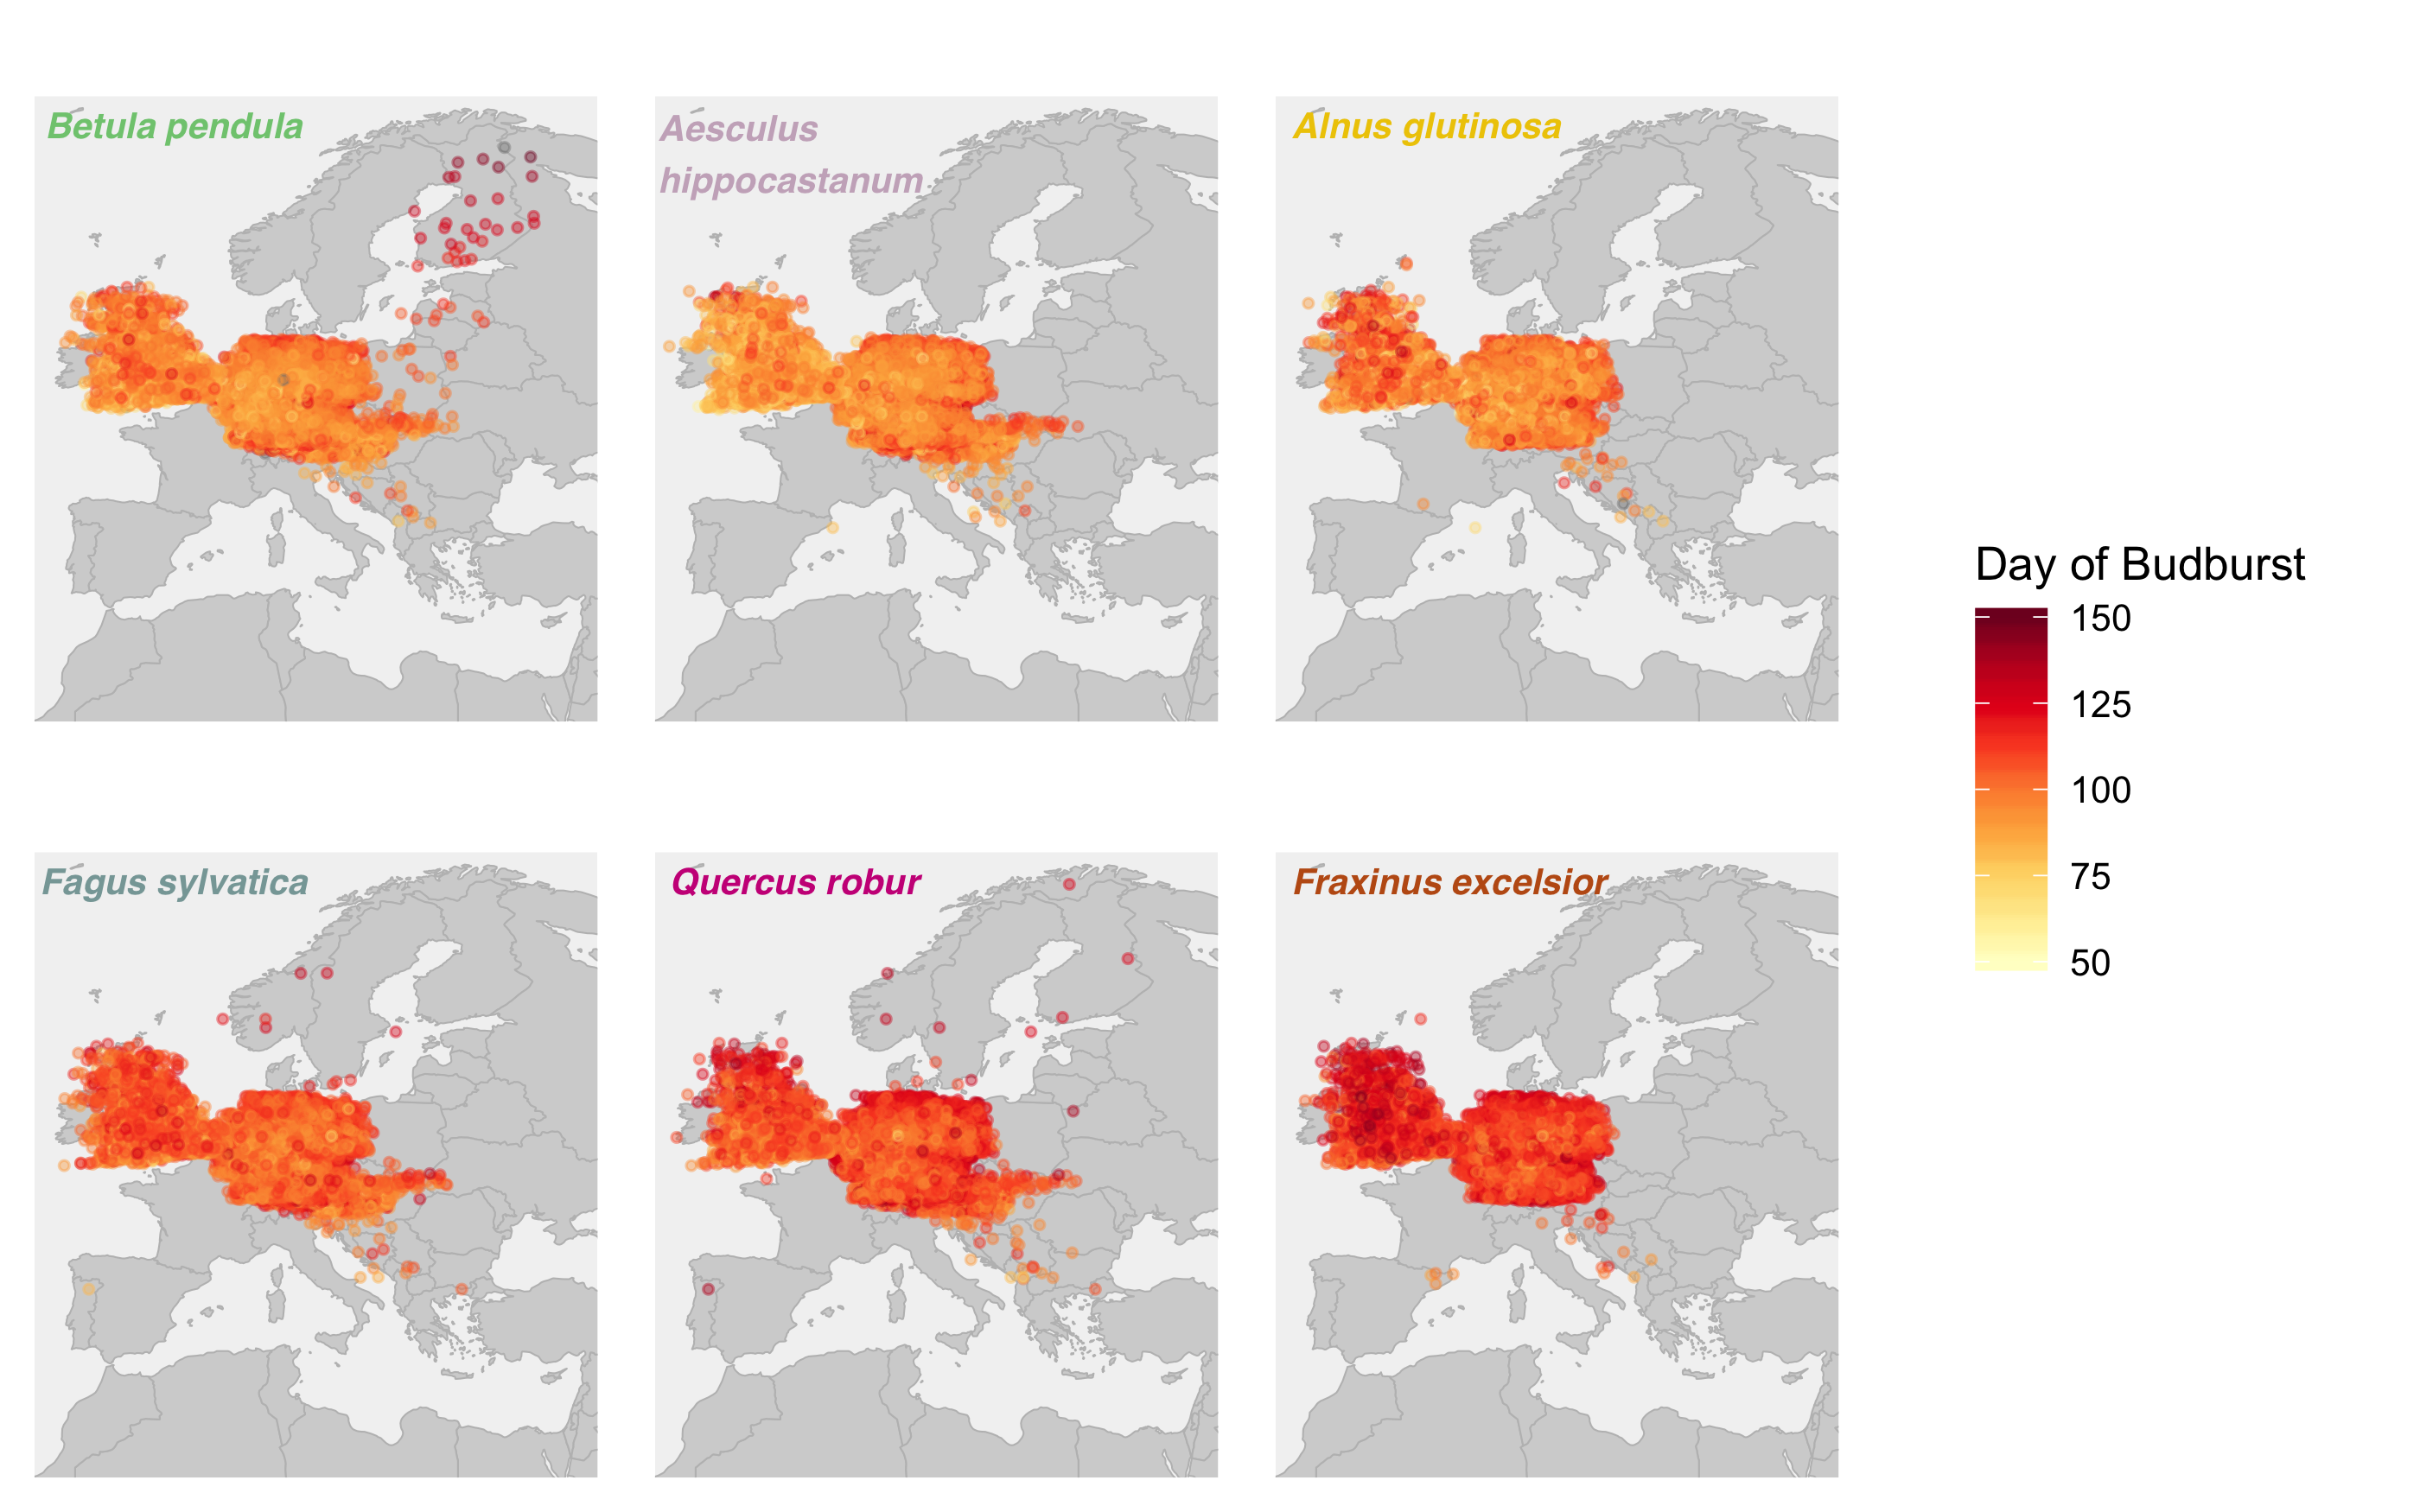
\includegraphics[width=14cm]{..//analyses/figures/BB_base.png}
  -\caption{The average day of budburst mapped by site for each species (ordered by day of budburst starting with \textit{Betula pendula} as the earliest budburst date to \textit{Fraxinus excelsior}). Species names are color-coded to match figures throughout the text. }\label{fig:bbmap}
  -\end{center}
  -\end{figure}}
  % Earlier budburst dates are yellow and later budburst dates are in red. % No need to repeat things shown on the graph generally.
  
{\begin{figure} [H]
  -\begin{center}
  -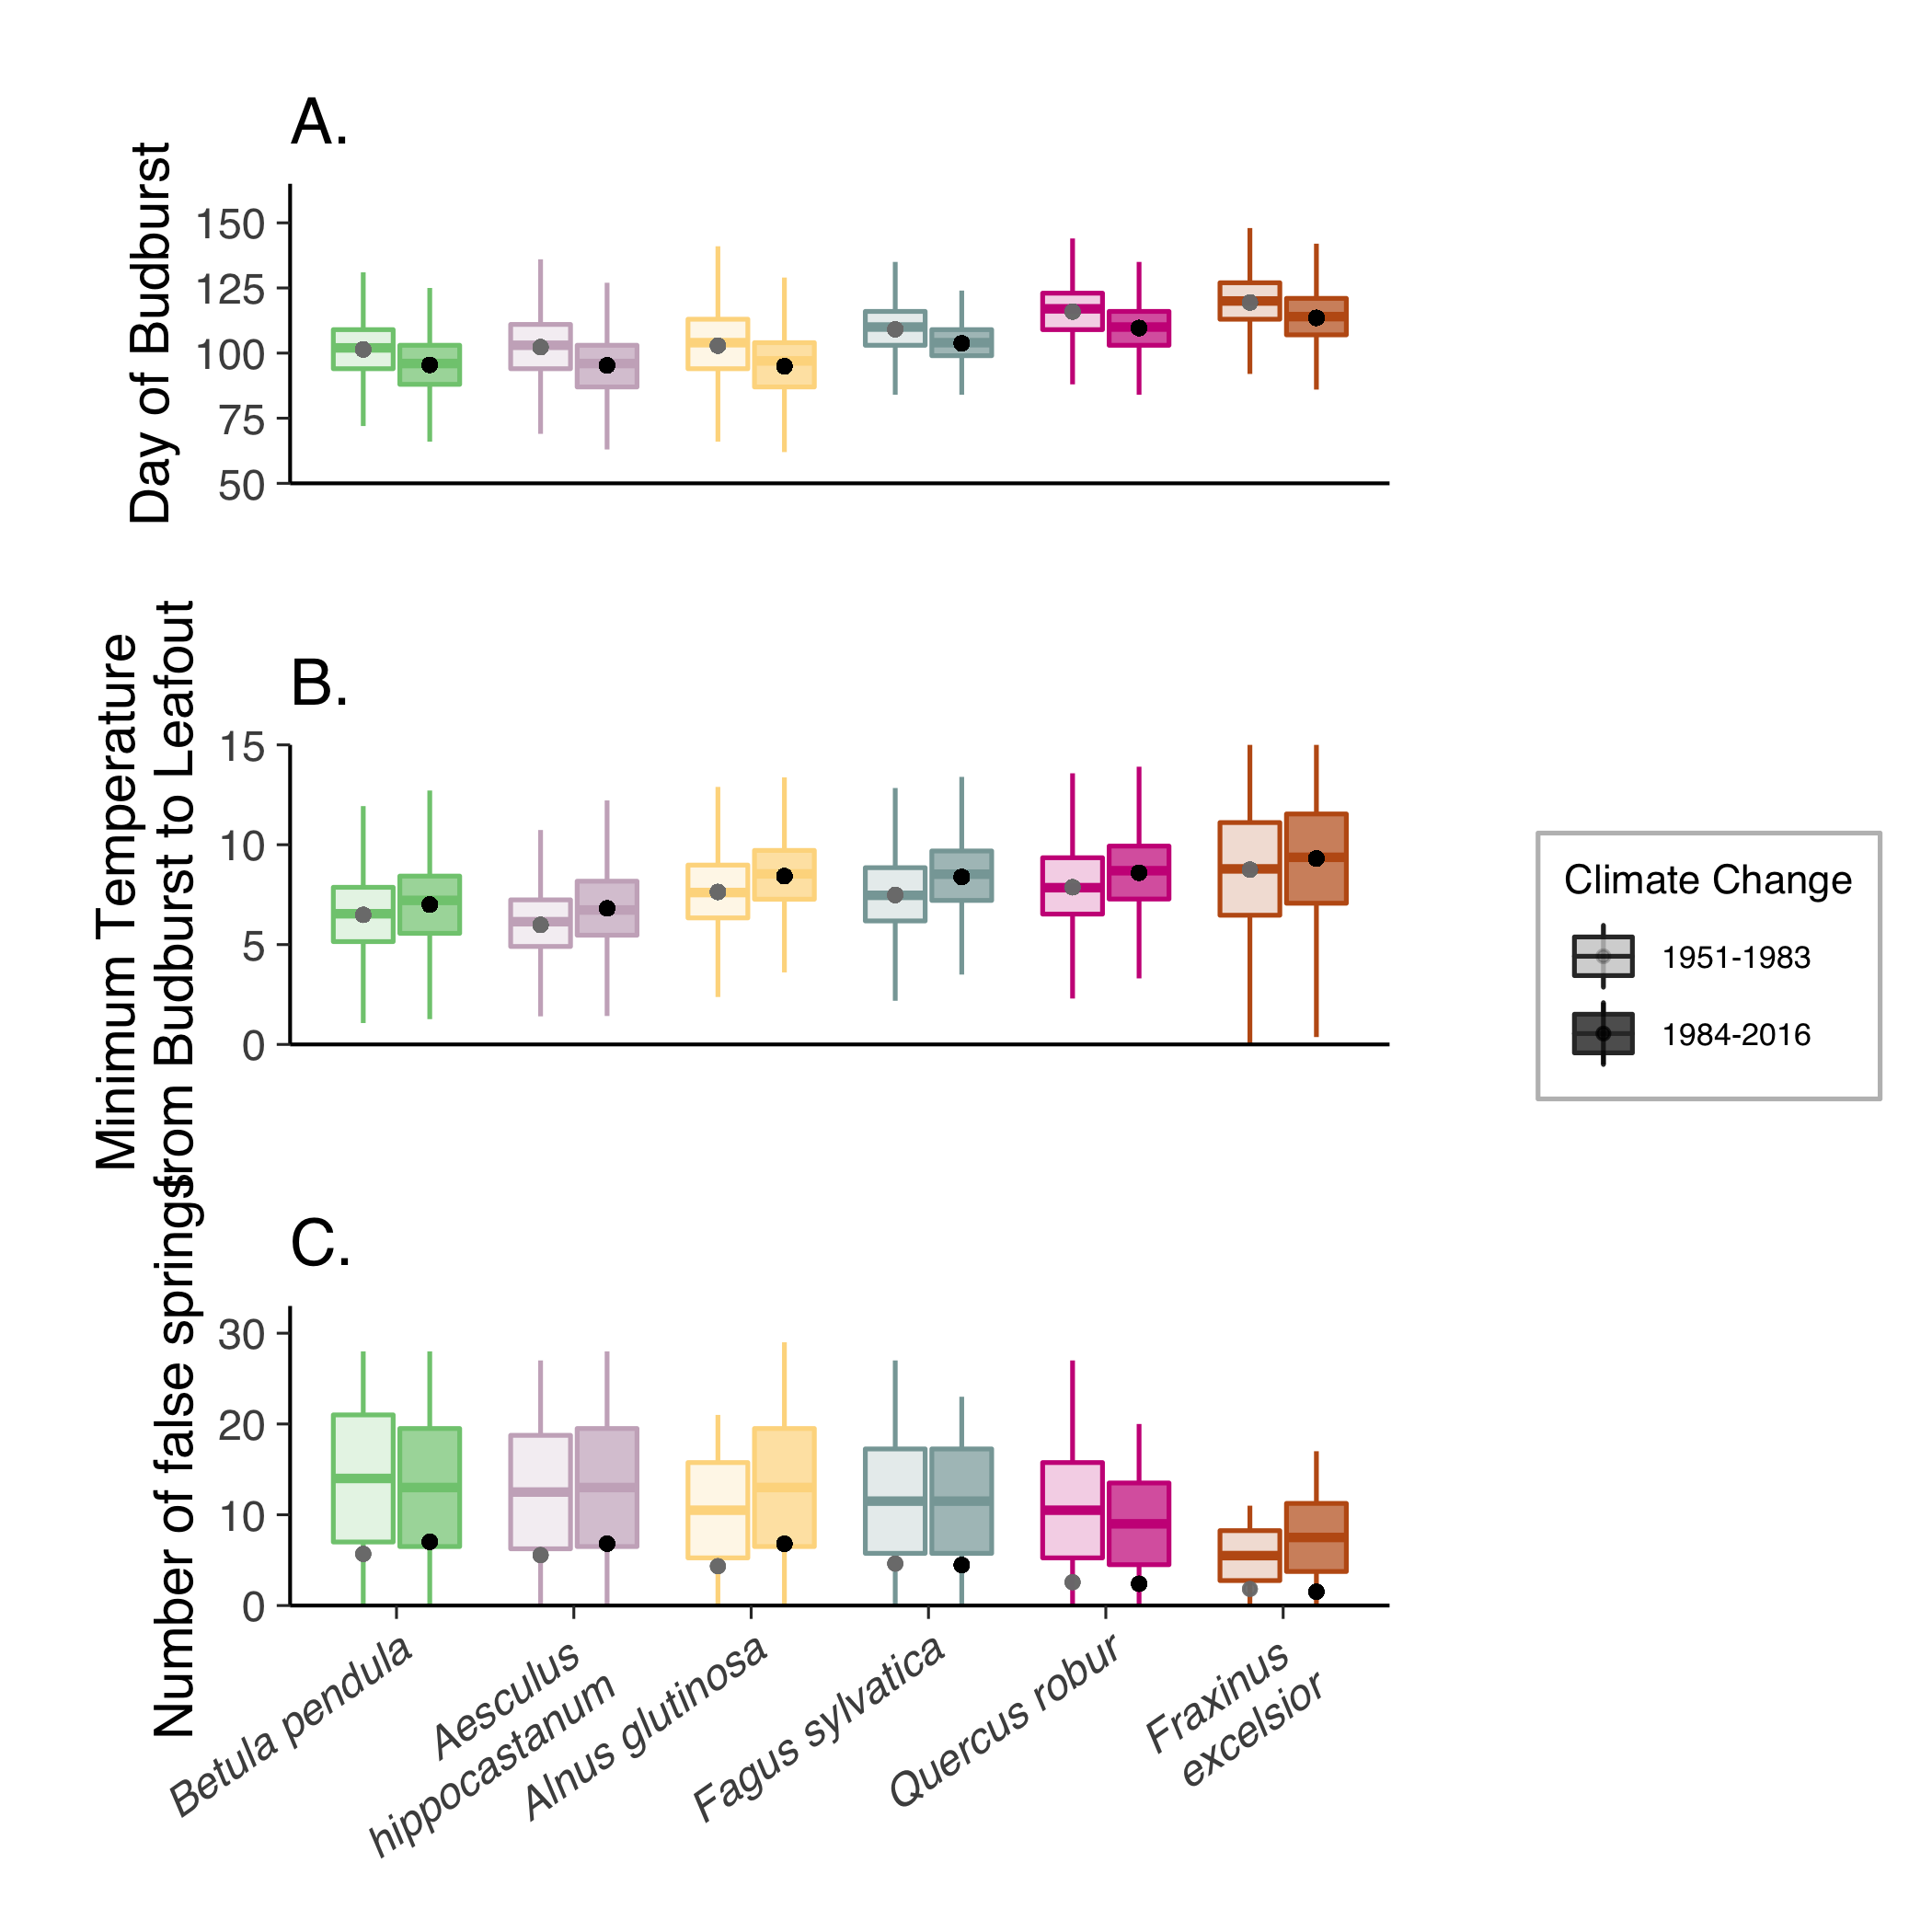
\includegraphics[width=14cm]{..//analyses/figures/Boxplot_BBTminFS_noDots_modests.png}
  -\caption{Day of budburst (A.), minimum temperatures between budburst and leafout (B.) and number of false springs (C.) before and after 1983 across species for all sites. Box and whisker plots show the 25th and 75th percentiles (i.e., the interquartile range) with notches indicating 95\% uncertainty intervals. Dots and error bars overlaid on the box and whisker plots represent the model regression outputs (Tables S3-S5). Error bars from the model regressions indicate 98\% uncertainty intervals but given the number of sites, which are quite small and thus not easily visible (see Table XX for more). Species are ordered by day of budburst and are color-coded to match the other figures.  }\label{fig:boxfs}
  % Are you sure the 'notches indicate 95\% uncertainty intervals'? If these are just plots of the RAW data then I am not sure how the box and whisker plots can generate uncertainty.... You generally need a model for that.
  -\end{center}
  -\end{figure}}
  
  
{\begin{figure} [H]
  -\begin{center}
  -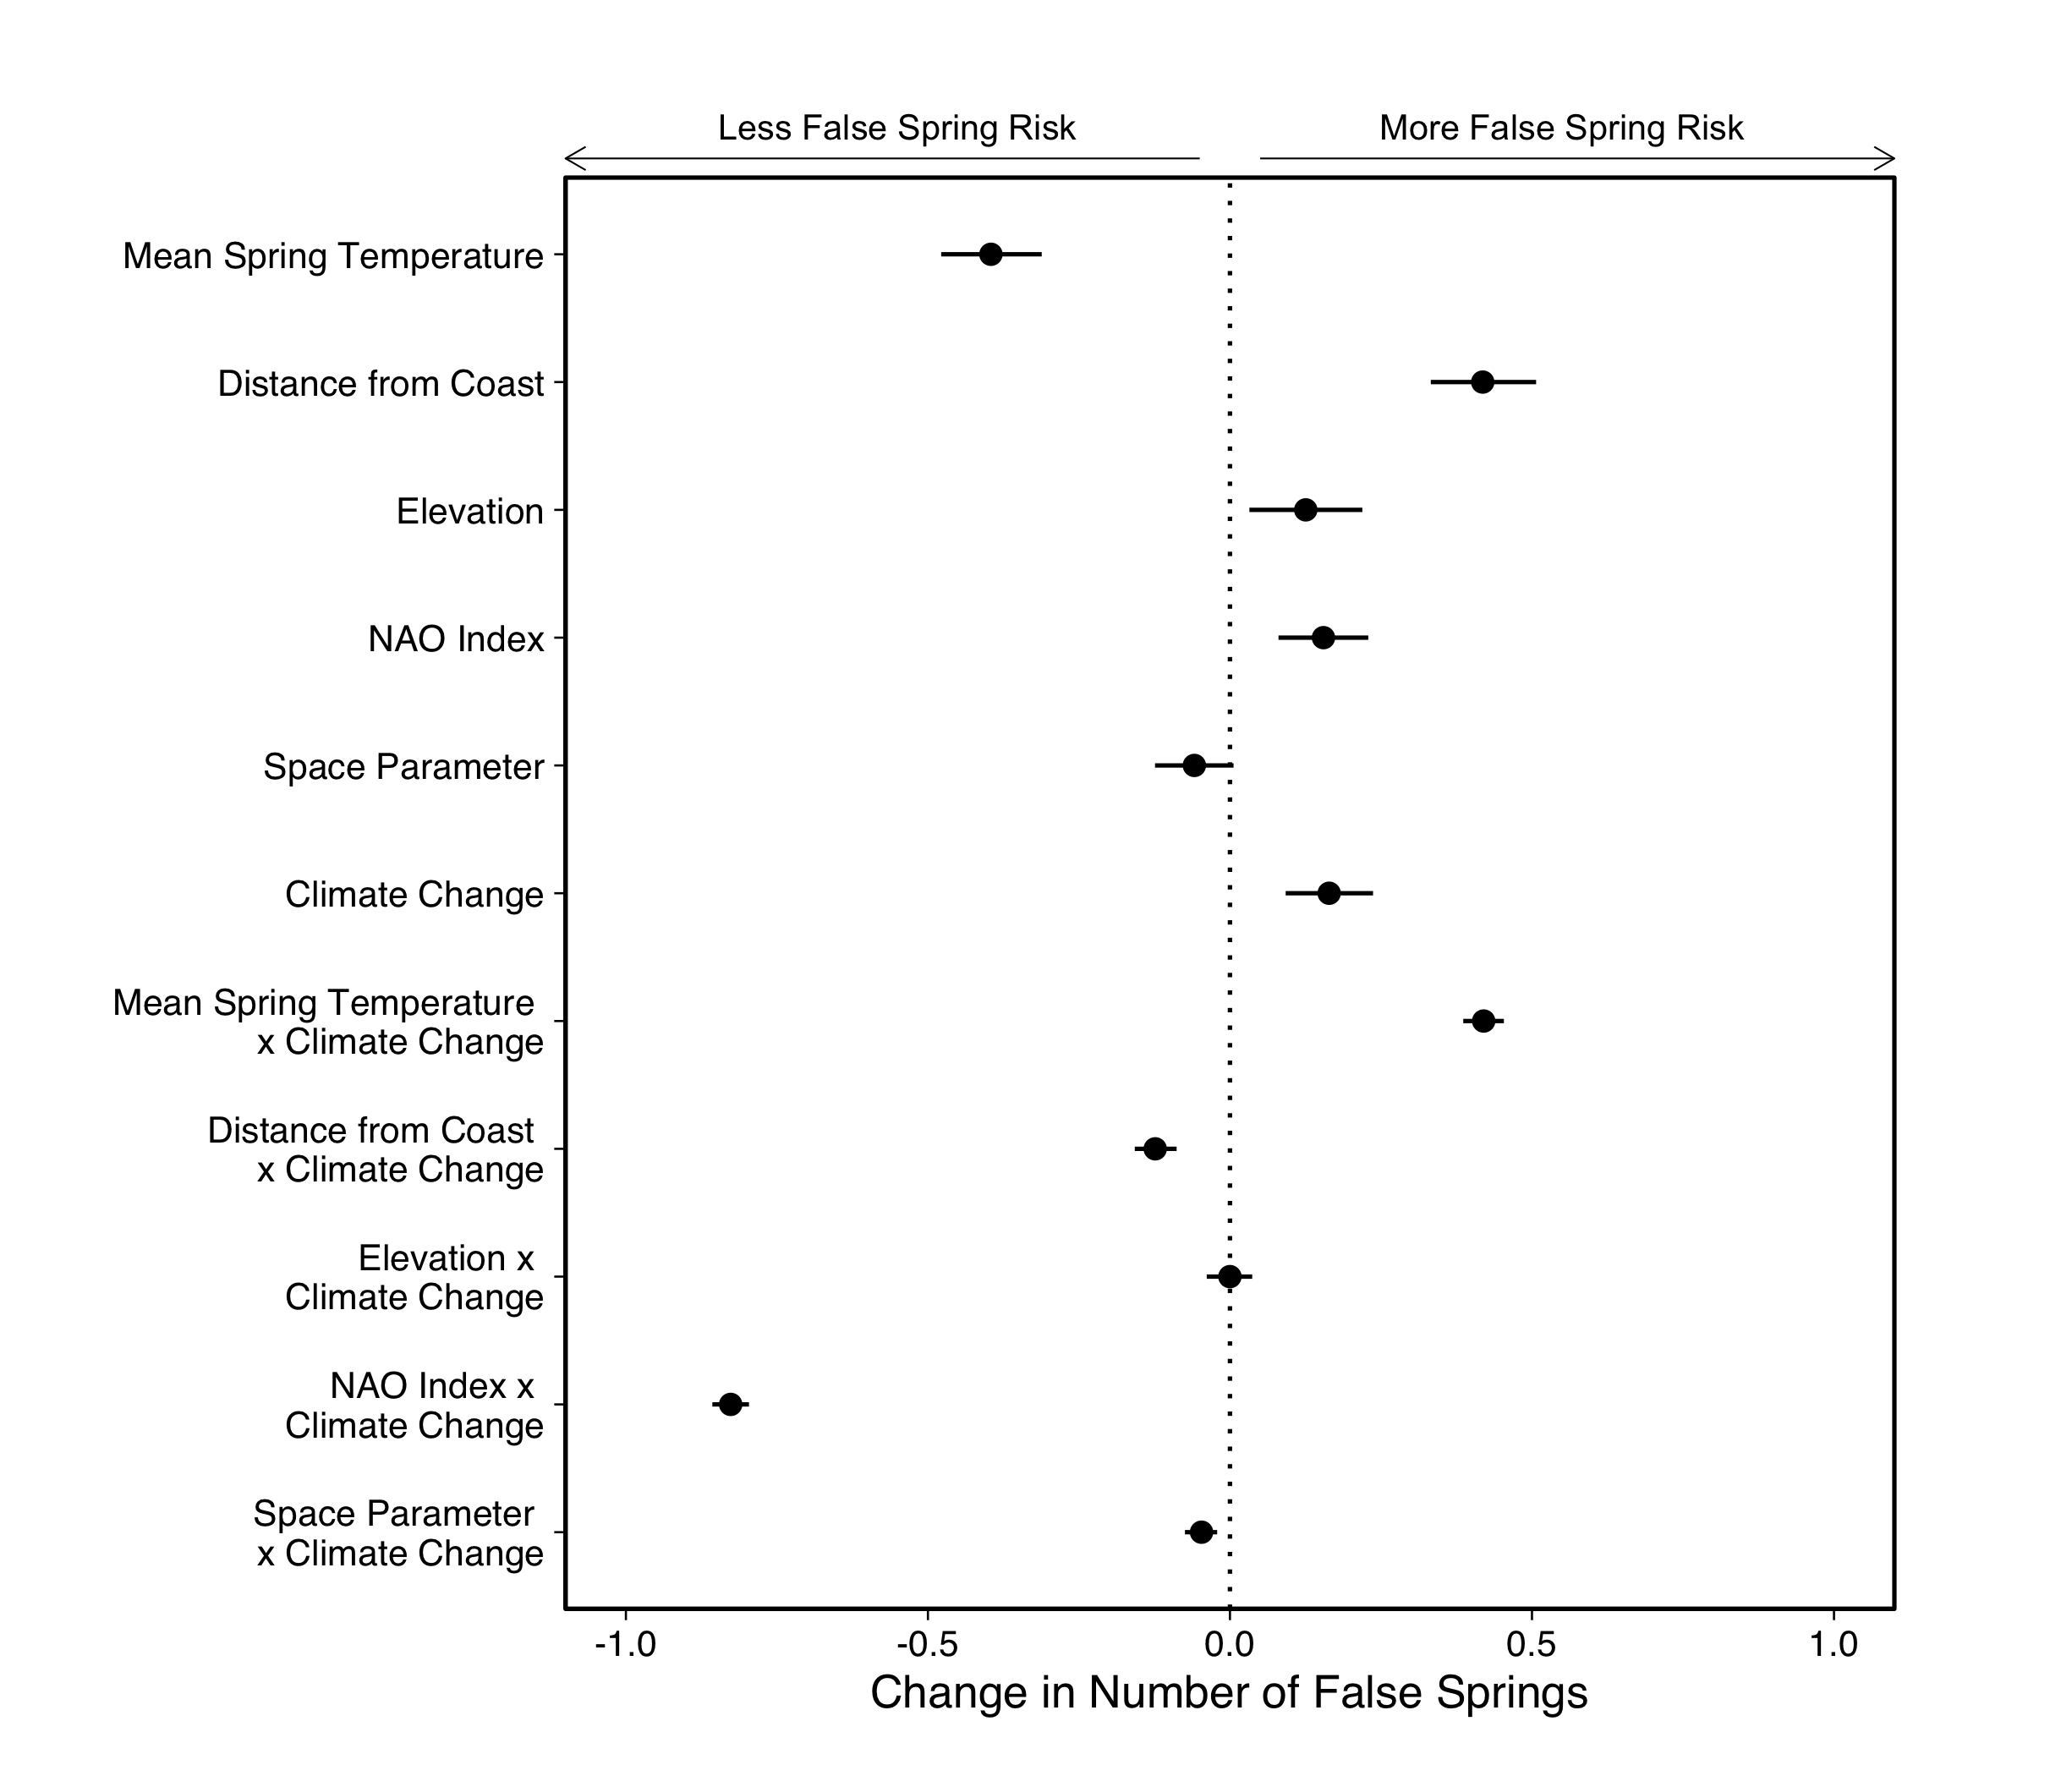
\includegraphics[width=12cm]{..//analyses/figures/model_output_98_orig.png}
  -\caption{Effects of species, climatic and geographical predictors on false spring risk. More positive values indicate an increased probability of a false spring whereas more negative values suggest a lower probability of a false spring. Dots and lines show means and 98\% uncertainty intervals. Values closer to zero have less of an effect on false springs. There were 582,211 zeros and 172,877 ones for false springs in the data.}\label{fig:maineffects}
  -\end{center}
  -\end{figure}}
  
{\begin{figure} [H]
  -\begin{center}
  -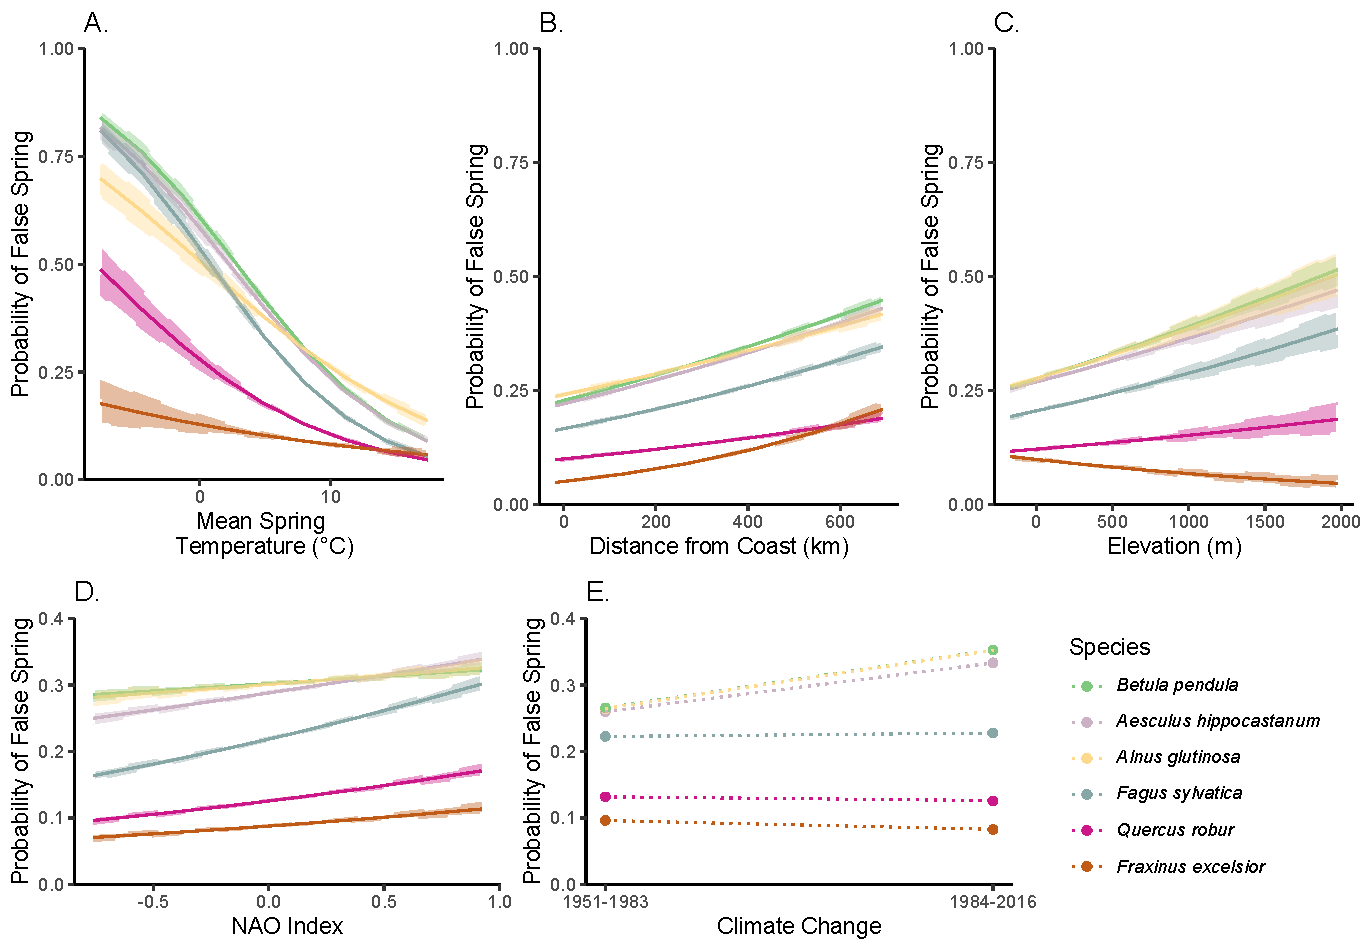
\includegraphics[width=16cm]{..//analyses/figures/InteractionPlots/Species_orig_98.pdf}
  -\caption{Species-level variation across geographic and spatial predictors (i.e., mean spring temperature (A.), distance from the coast (B.), elevation (C.), and NAO index (D.)). Lines and shading are the mean and 98\% uncertainty intervals for each species. To reflect the raw data, we converted the model output back to the original scale for the x-axis in each panel. }\label{fig:spp}
  -\end{center}
  -\end{figure}}
  
  \renewcommand{\thefigure}{S1}
  {\begin{figure} [H]
  -\begin{center}
  -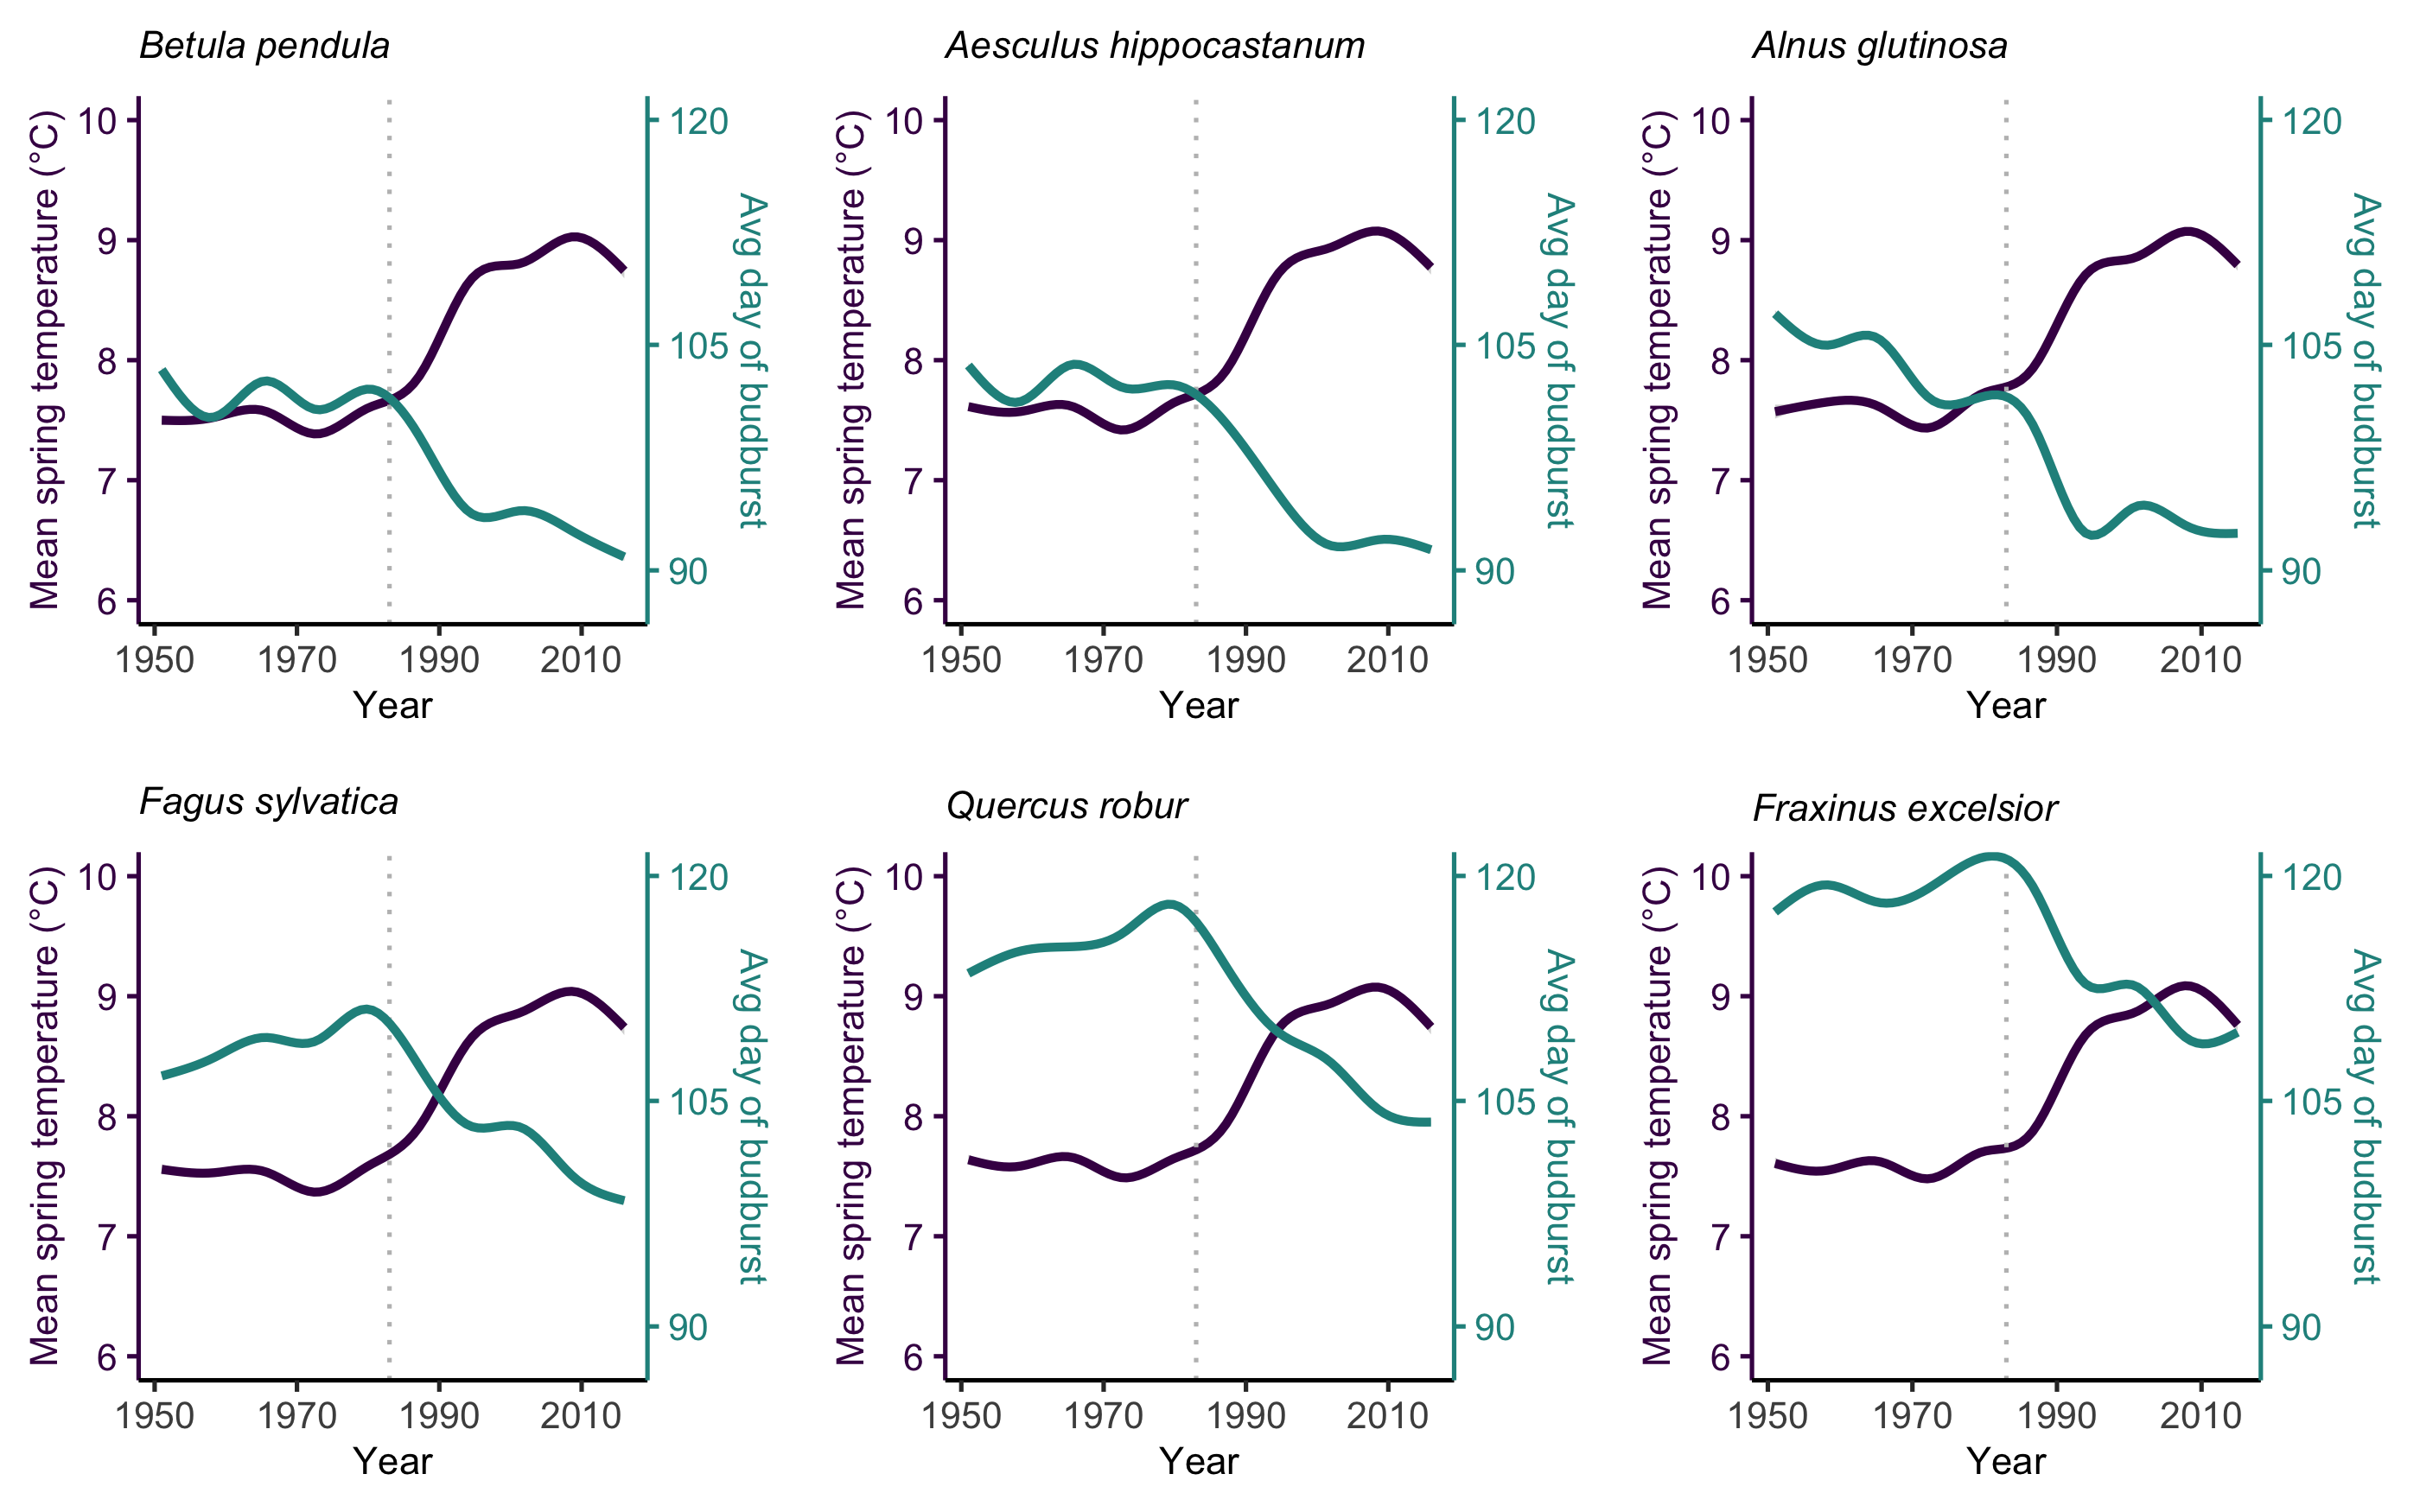
\includegraphics[width=16cm]{..//analyses/figures/MSTBB_bySpp_lines.png}
  -\caption{Mean spring temperatures are plotted for each site and year (from 1951-2016) for each species. The purple line shows the trend in mean spring temperatures from March 1 to May 31 and the green line represents the trend of average day of budburst for each year for each species. Both lines are cyclic penalized cubic regression spline smooths with basis dimensions equal to the number of years in the study (i.e., 66). Species are ordered by average day of budburst, with the earliest being \textit{Betula pendula} and the latest being \textit{Fraxinus excelsior}. }\label{fig:mst}
  -\end{center}
  -\end{figure}}


\end{document}
